\section{Viewing}
\textit{von 3D in 2D abbilden}

\subsection{Planare geometrische Projektionen}
\textit{Bild auf eine Ebene projezieren}

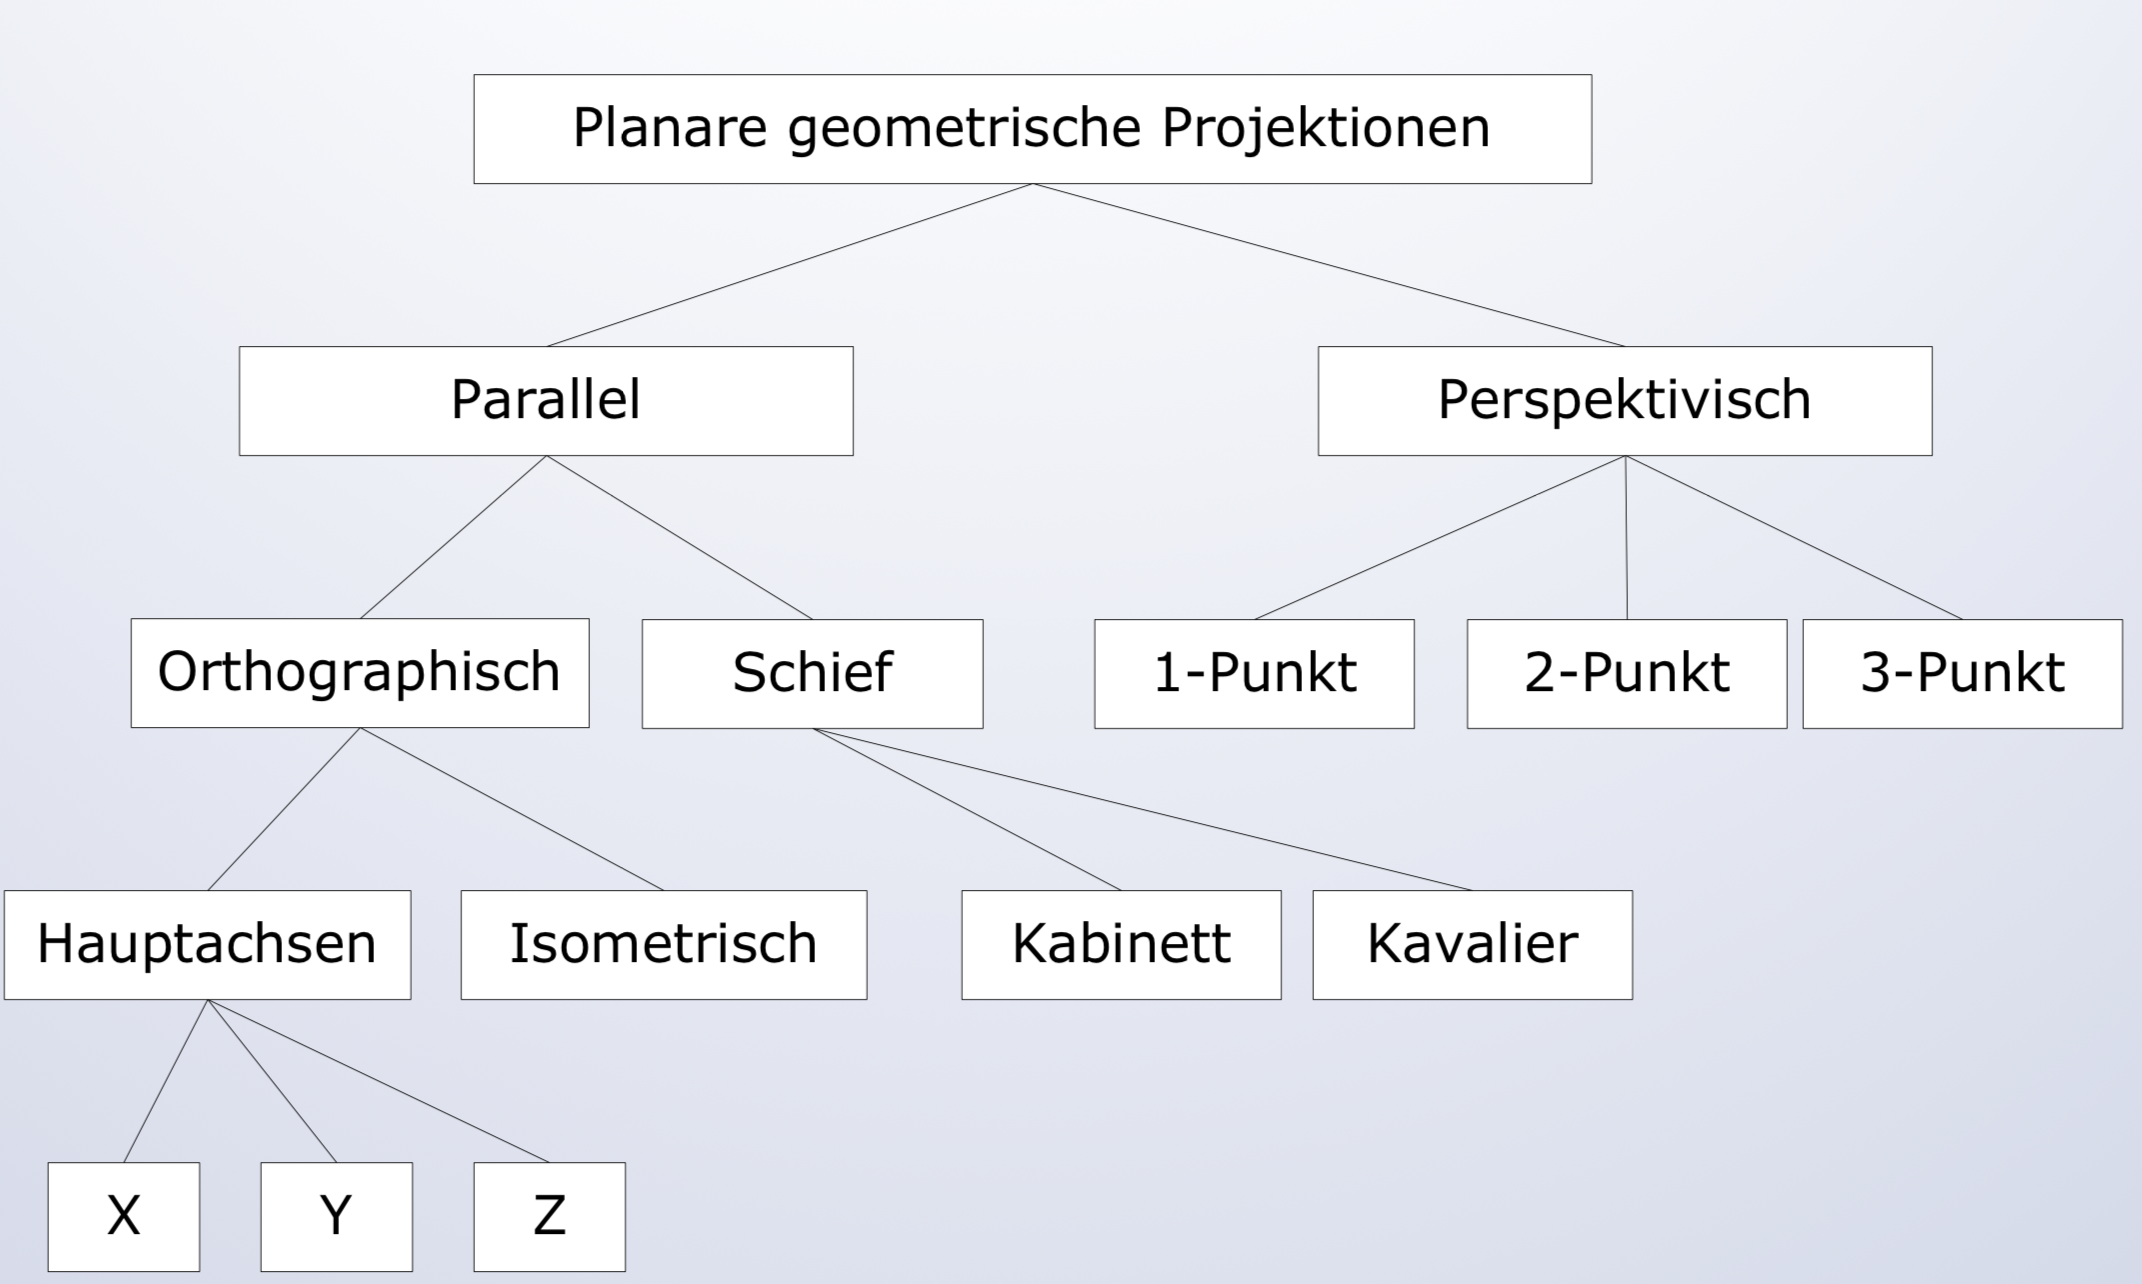
\includegraphics[width=0.45\textwidth]{assets/KlassifikationvonProjektionen.png}

\subsubsection{paralelle Projektionen}

\begin{itemize}
    \item Geraden und Parallelen bleiben erhalten
    \item konstante Verkürzung in eine Richtung
    \item keine Winkeltreue
\end{itemize}

\paragraph{Ortographische Projektion}
\textit{von einer Seite / rechtwinklig}\\
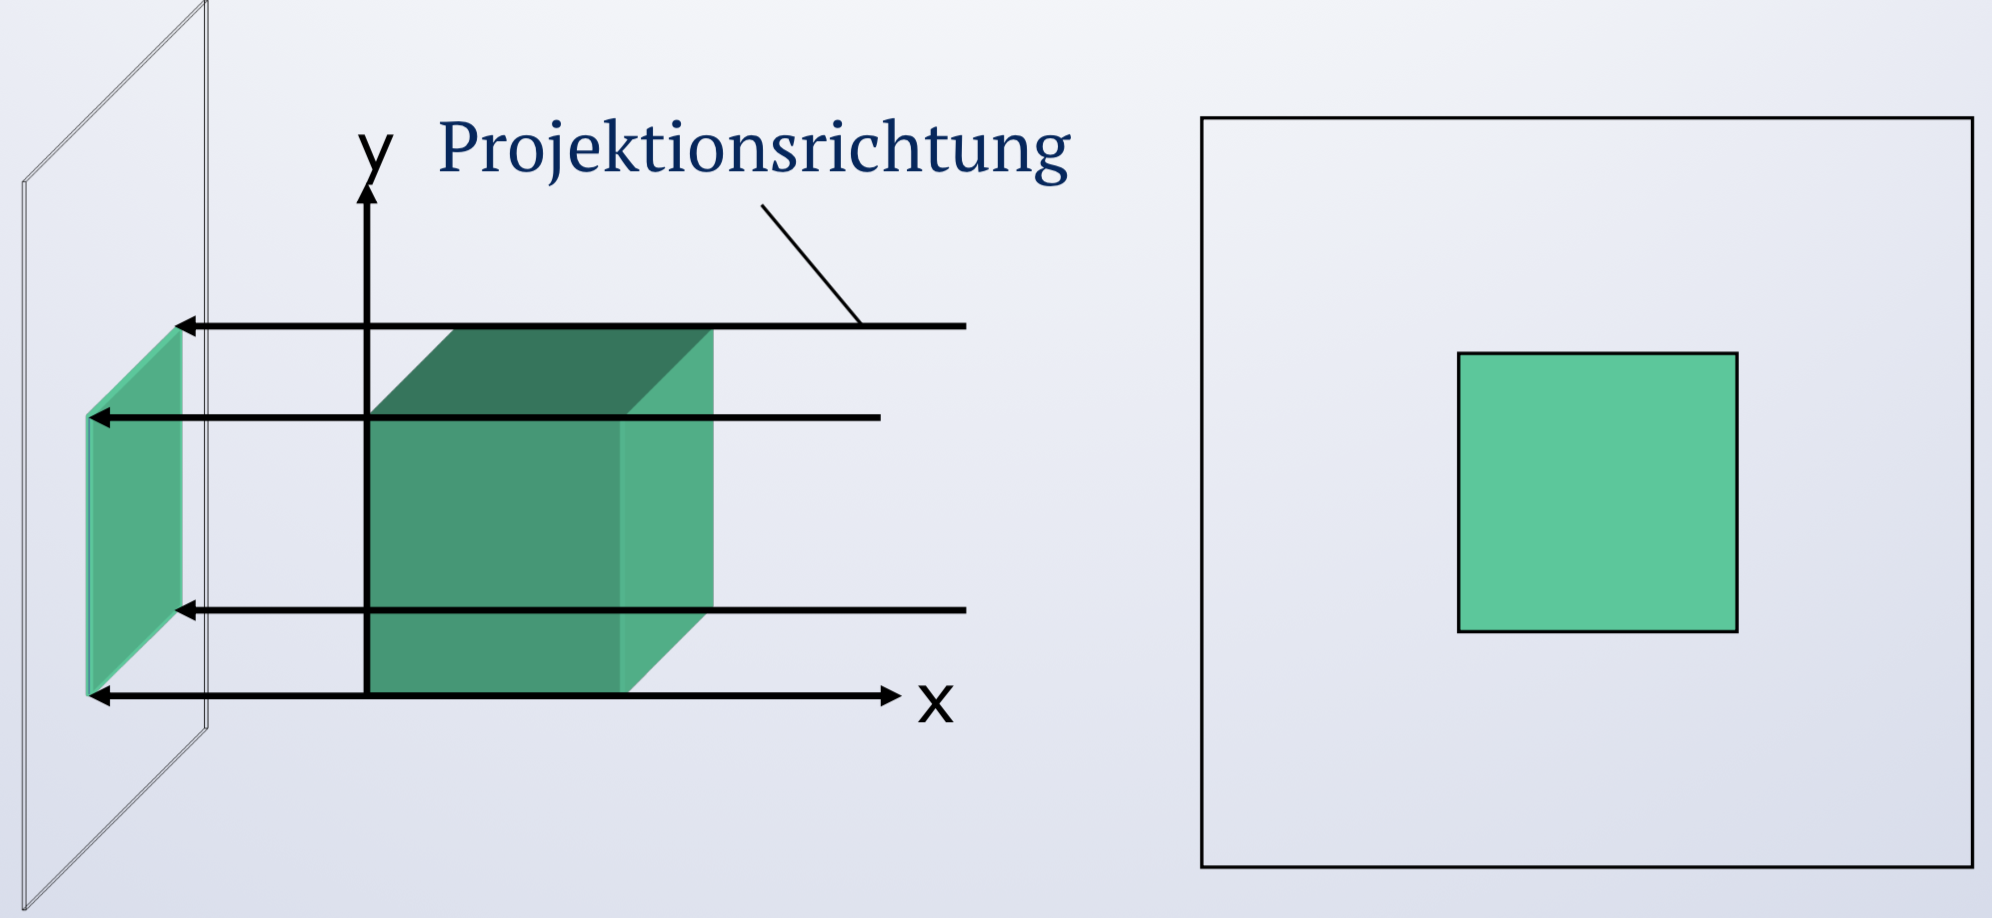
\includegraphics[width=0.25\textwidth]{assets/OrtographischeProjektion.png}

\paragraph{Isometrische Projektion}
\textit{Ortographische auf die Ebene (1,1,1)}\\
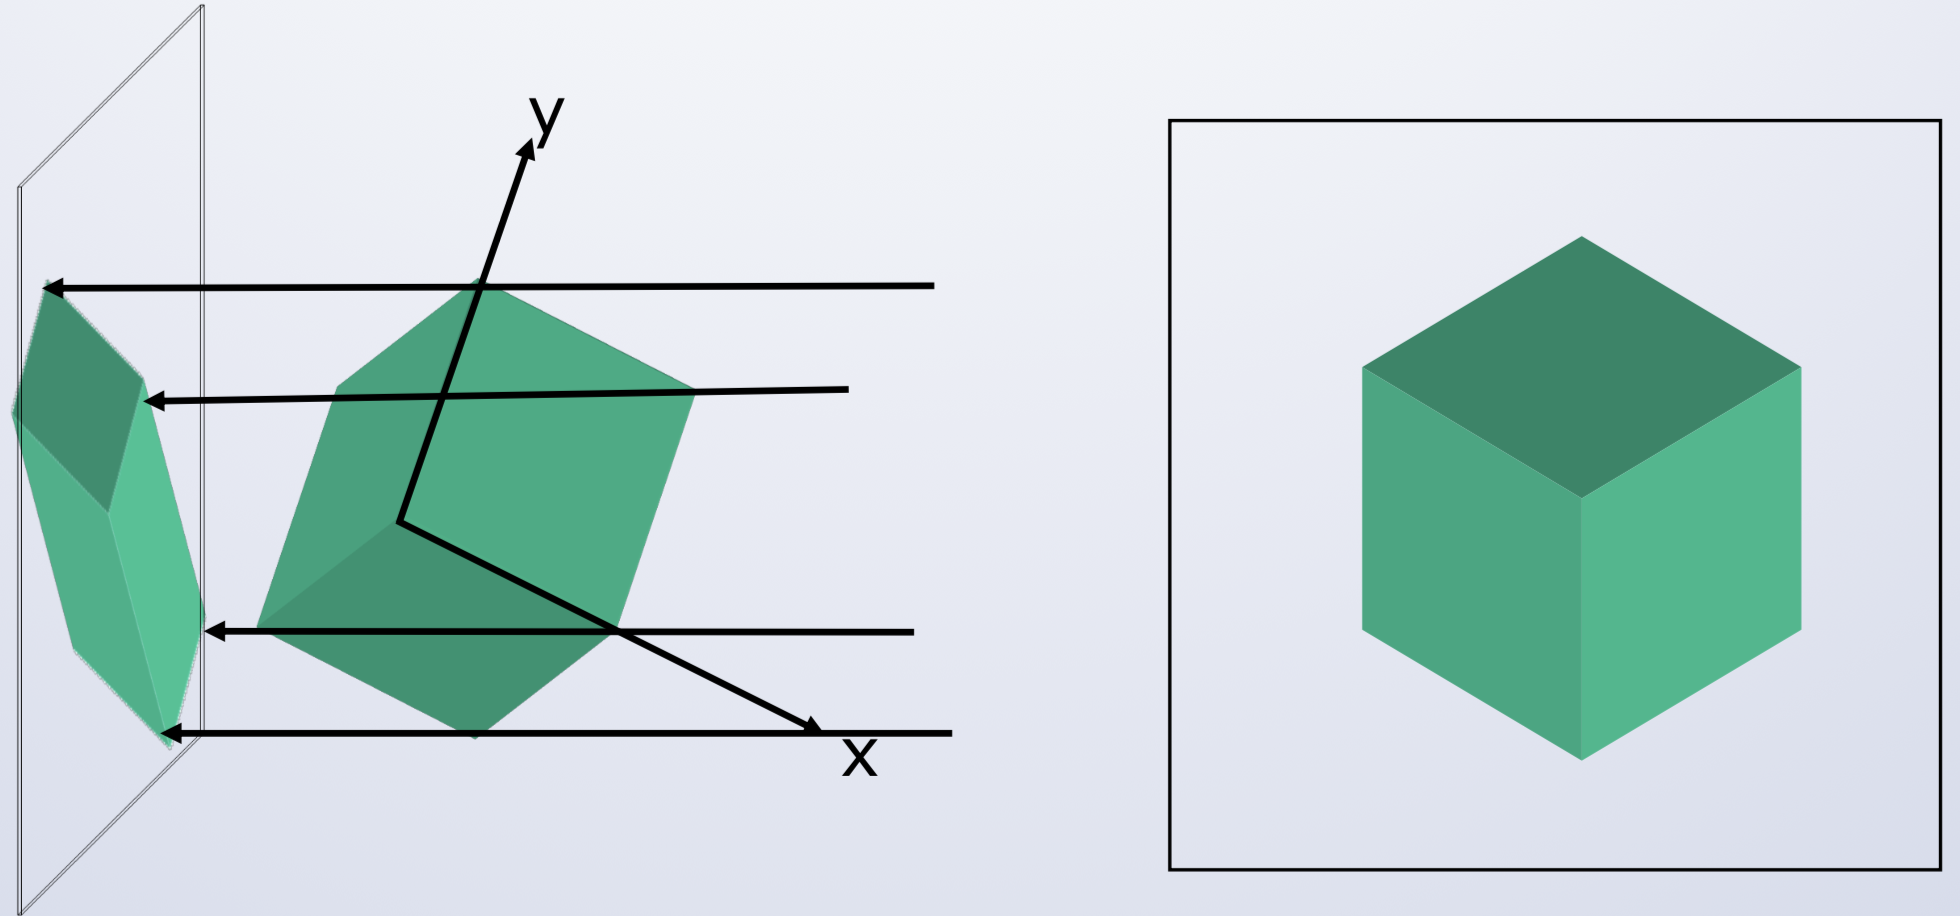
\includegraphics[width=0.25\textwidth]{assets/IsometrischeProjektion.png}

\paragraph{Kavaliersprojektion}
\textit{Parallelprojektion mit 45 Grad. Linien rechtwinklig zur Ebene haben natürliche Länge}\\
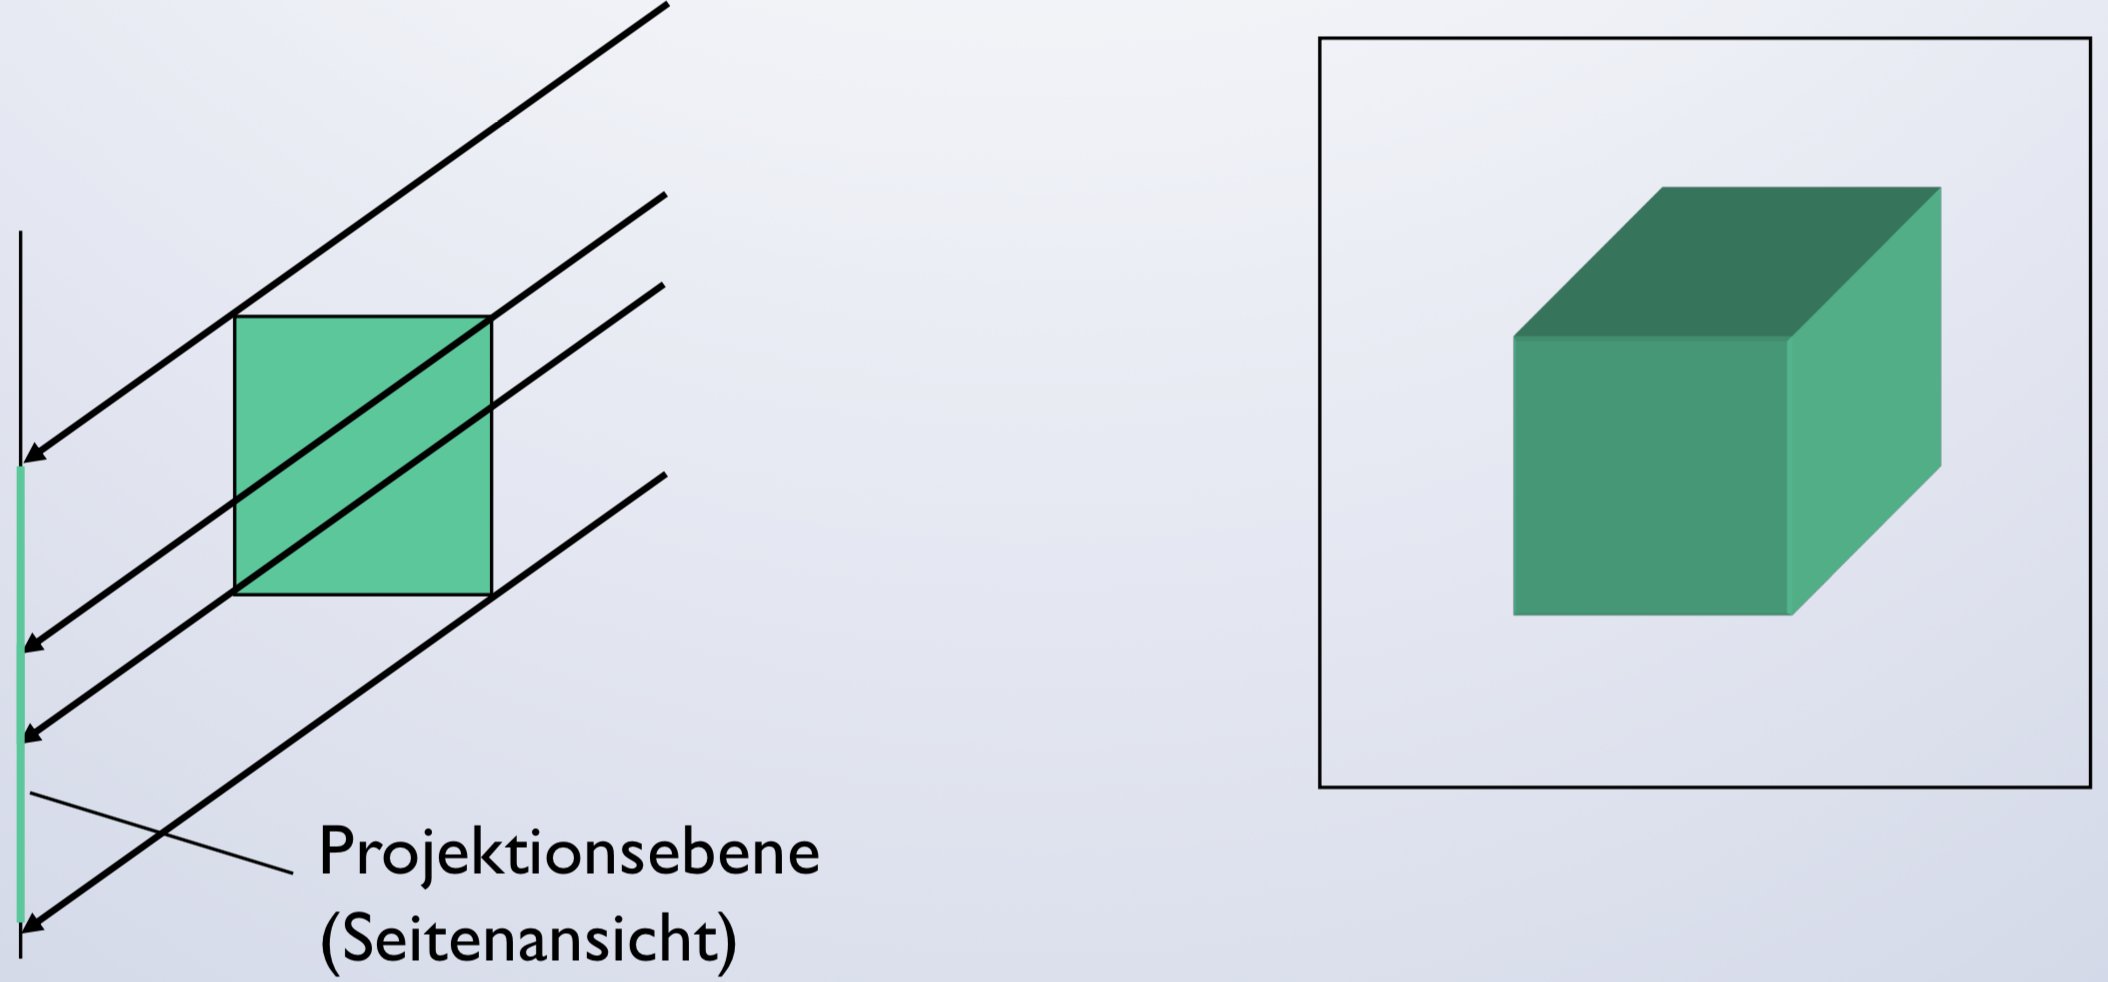
\includegraphics[width=0.25\textwidth]{assets/Kavaliersprojektion.png}

\paragraph{Kabinettsprojektion}
\textit{Parallelprojektion mit 63.4 Grad. Linien rechtwinklig zur Ebene haben halbe Länge}\\
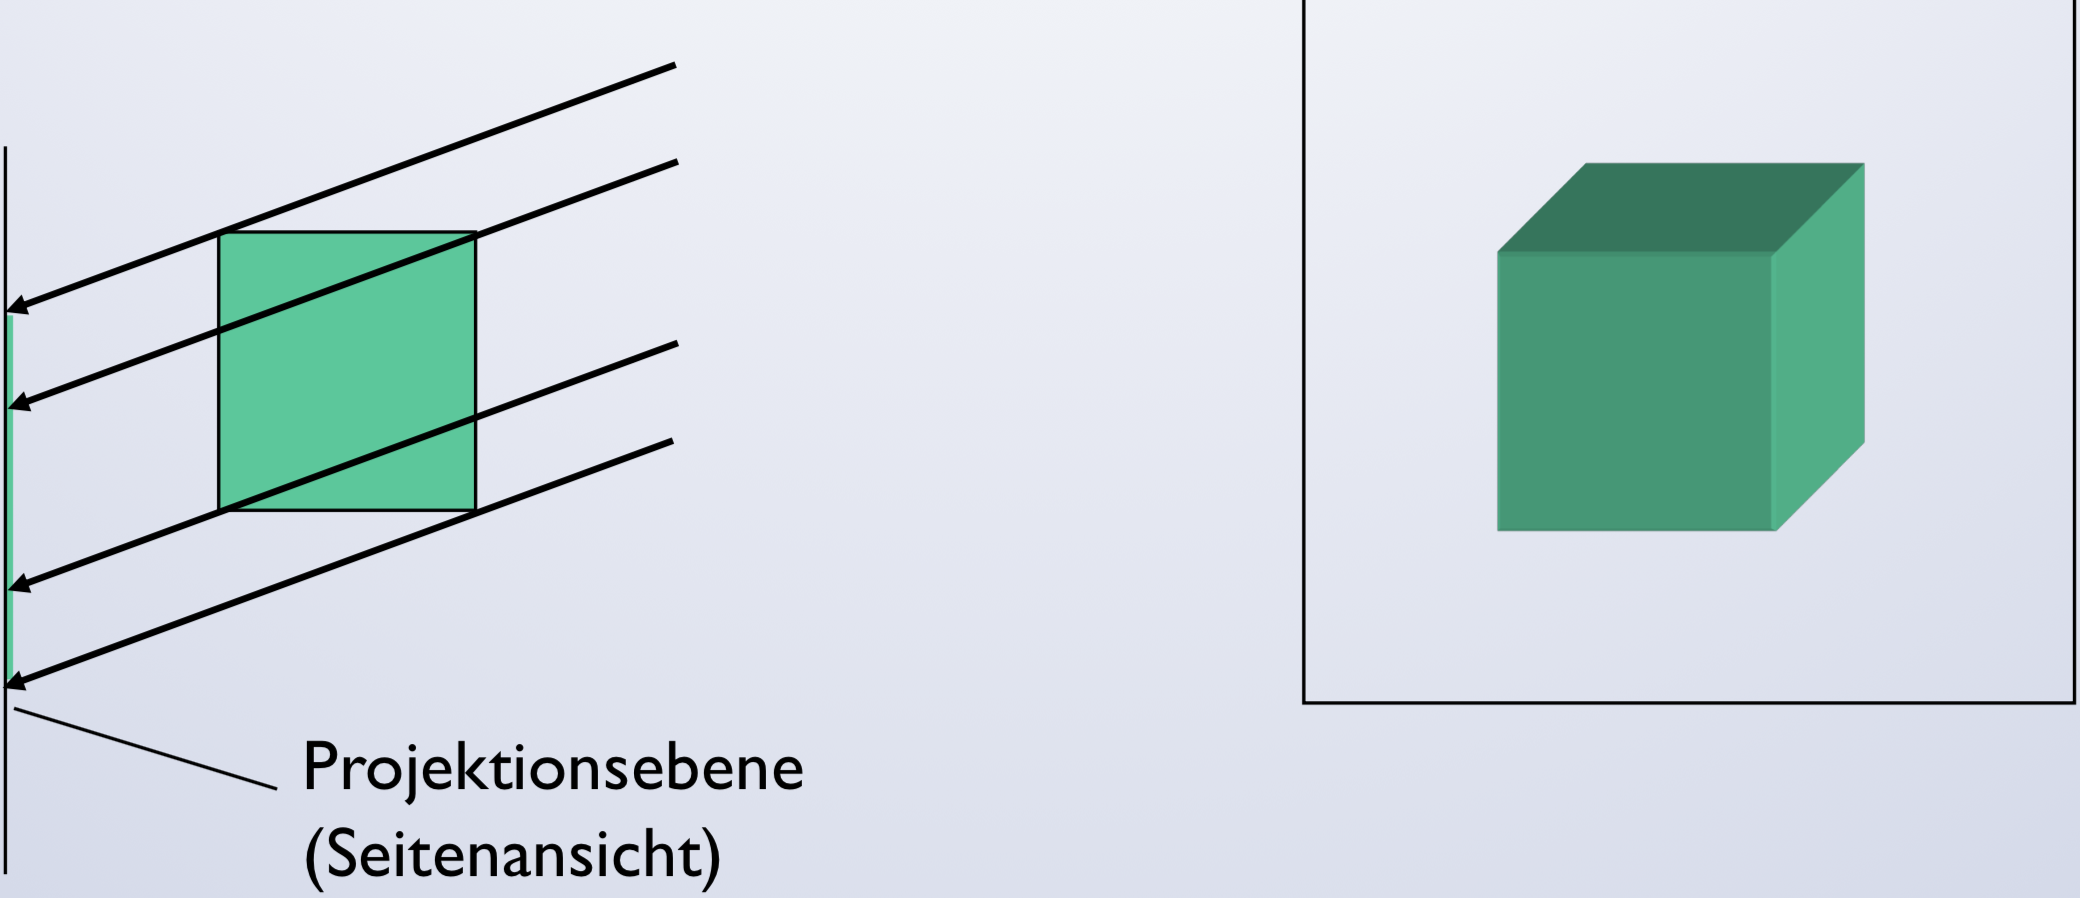
\includegraphics[width=0.25\textwidth]{assets/Kabinettsprojektion.png}

\subsubsection{perspektivitsche Projektionen}
\begin{itemize}
    \item Simuliert Kamera oder Auge
    \item Spezifiziert durch Projektionszentrum und Projektionsebene
    \item Geraden bleiben erhalten
    \item Parallelen schneiden sich in einem Punkt (Fluchtpunkt)
    \item Objektgrösse nimmt proportional zum Abstand vom Projektionszentrum ab
\end{itemize}
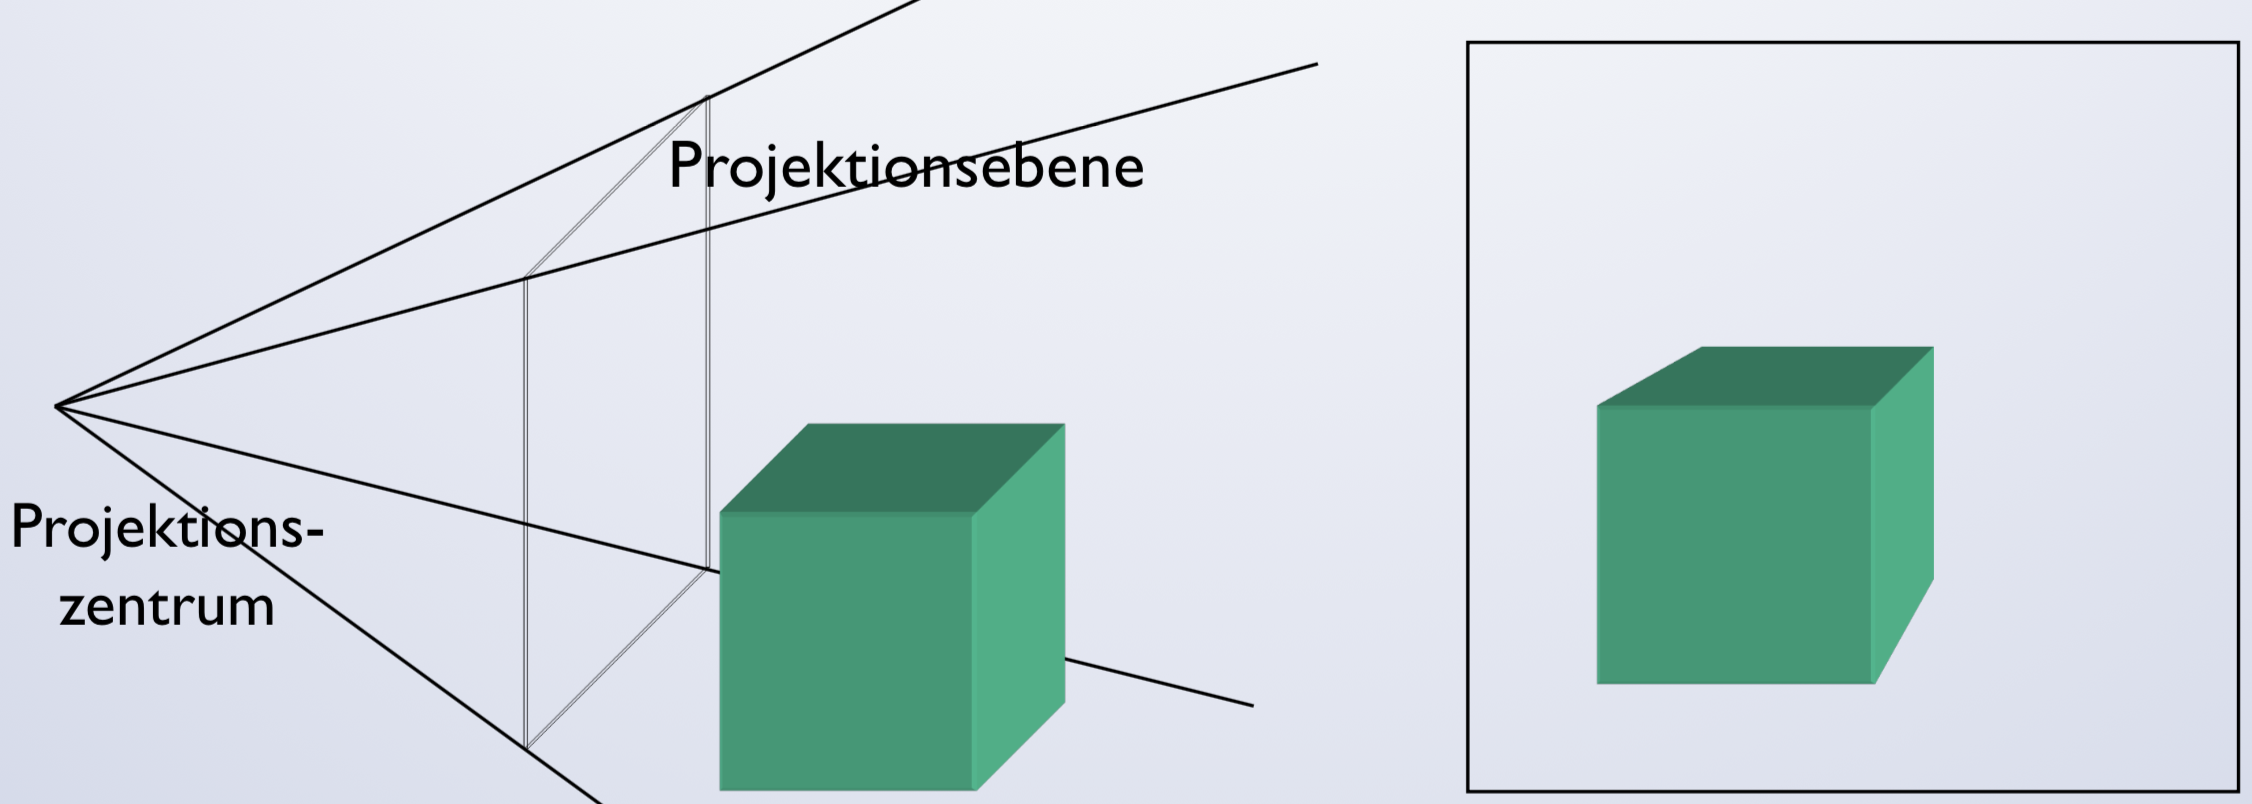
\includegraphics[width=0.35\textwidth]{assets/perspektivische-projektion.png}

\subsubsection{perspektivitsche Projektion berechnen}

\textit{Projektionsebene parallel zur x-y Ebene bei z=d wenn Projektionszentrum = $(0,0,0)$} \\

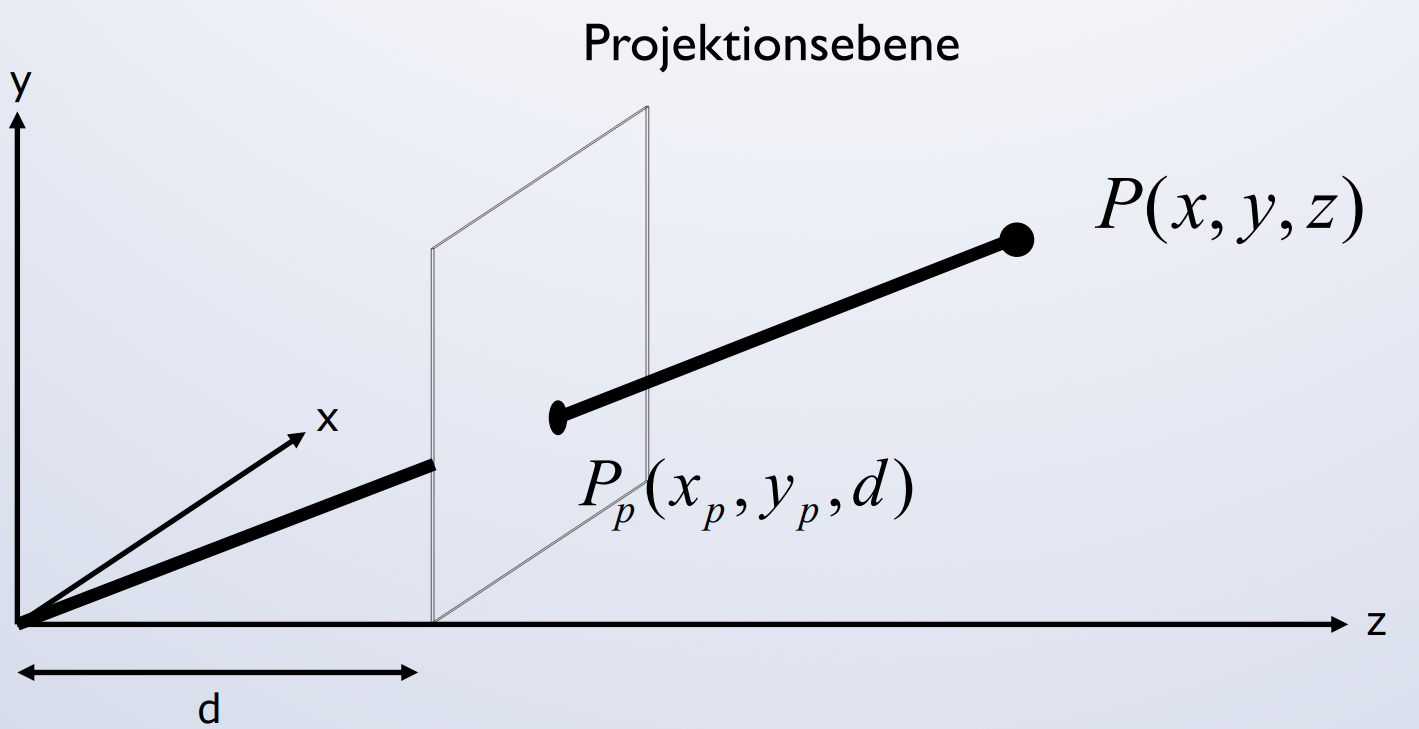
\includegraphics[width=0.4\textwidth]{assets/viewing-projektionsebene.png}

\textit{Ansicht entlang x-Achse}

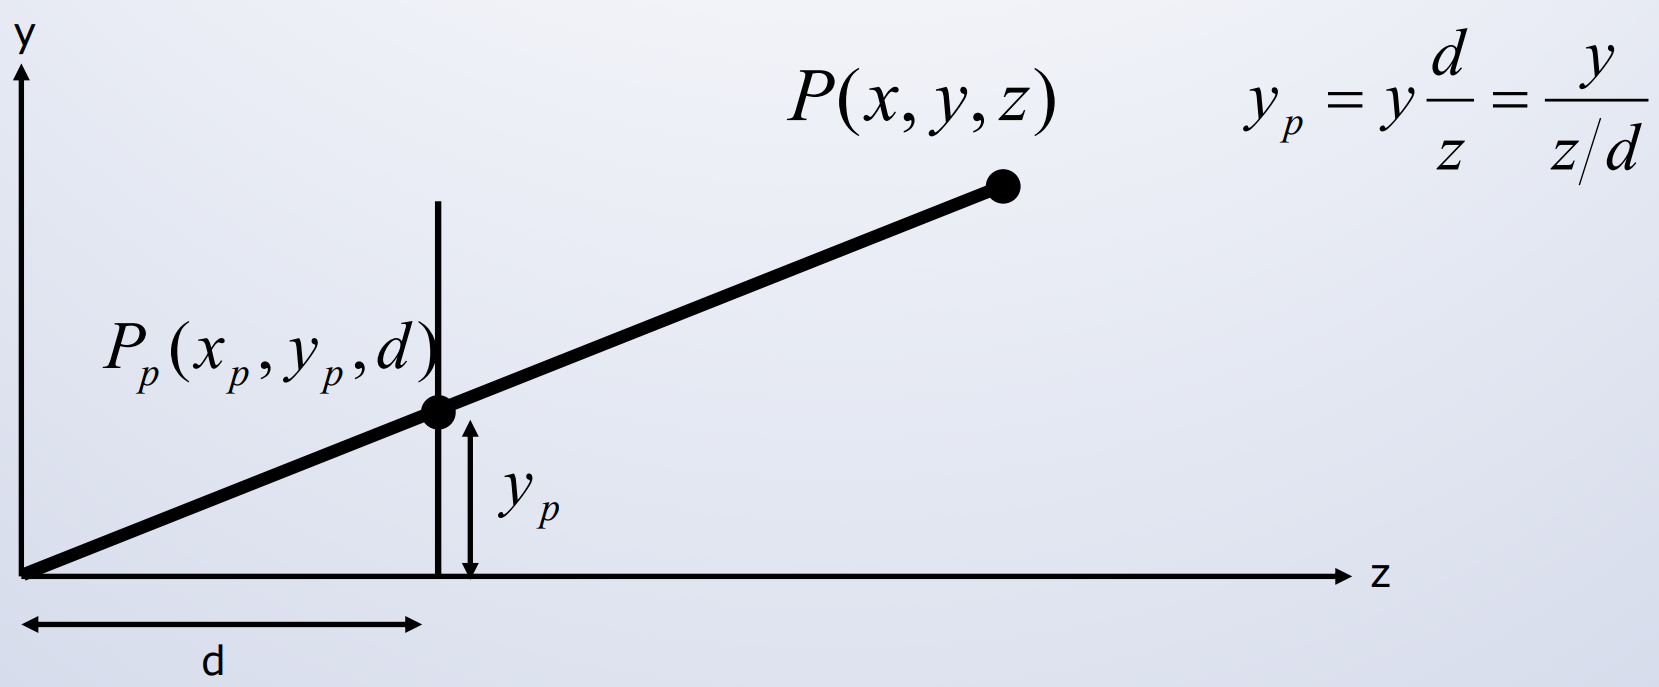
\includegraphics[width=0.4\textwidth]{assets/viewing-projektionsebene-xachse.png}

\textit{Projektionsmatrix in homogene Koordinaten}\\
$M_{per} = \begin{bmatrix}
    1 & 0 & 0 & 0 \\
    0 & 1 & 0 & 0 \\
    0 & 0 & 0 & 0 \\
    0 & 0 & \frac{1}{d} & 1 \\
\end{bmatrix}$\\

\textit{Für $d \leftarrow \infty$ entsteht eine Parallelprojektionsmatrix}
$M_{orth}' = \begin{bmatrix}
    1 & 0 & 0 & 0 \\
    0 & 1 & 0 & 0 \\
    0 & 0 & 0 & 0 \\
    0 & 0 & 0 & 1 \\
\end{bmatrix}$

\subsection{Vertex Transformationen}

\textit{Matrix im Vertexshader benötigt:}

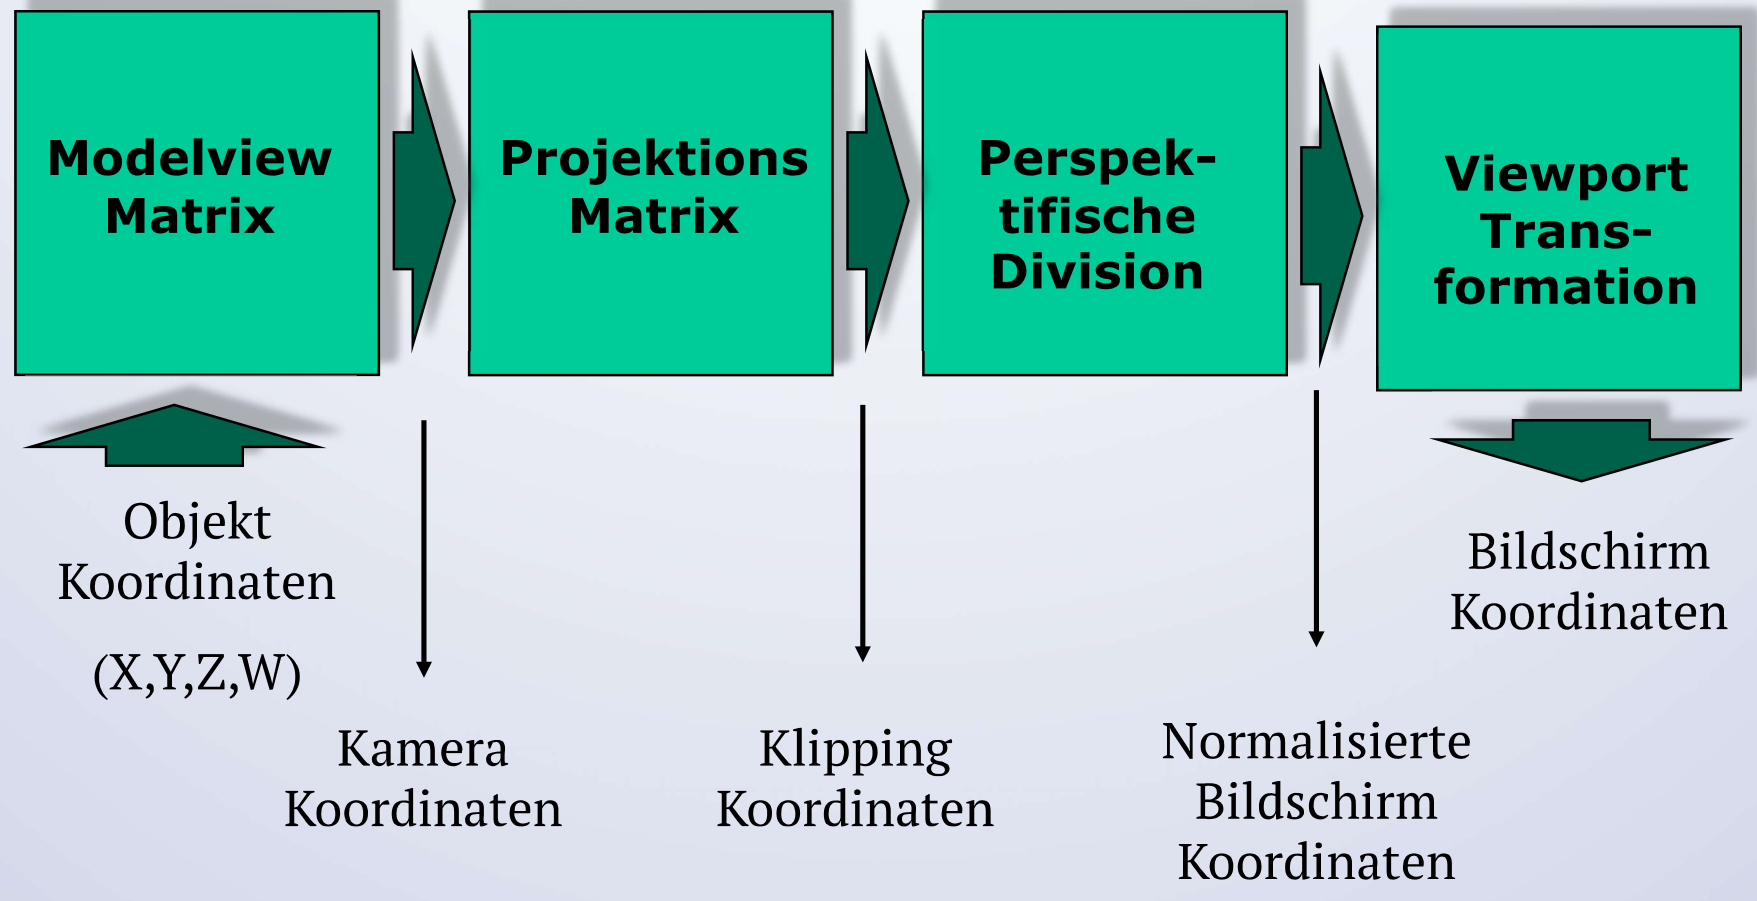
\includegraphics[width=0.4\textwidth]{assets/vertex-transformation.png}

\begin{lstlisting}
attribute vec3 aVertexPosition;
uniform mat4 uModelViewMatrix;
uniform mat4 uProjectionMatrix;
void main() {
  vec4 position = vec4(aVertexPosition, 1.0);
  gl_Position =
    uProjectionMatrix *
    uModelViewMatrix *
    position;
}
\end{lstlisting}


